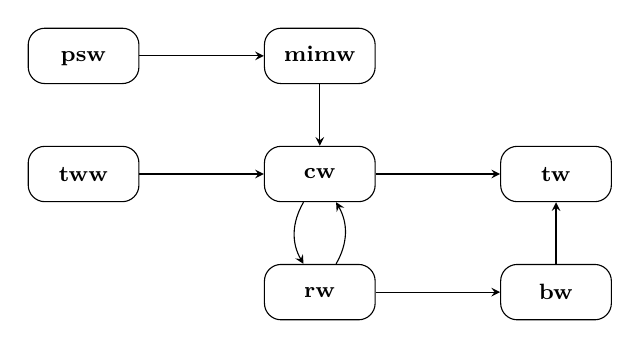
\begin{tikzpicture}[nodes=rectangle, nodes=draw, font=\footnotesize, minimum width=40pt, minimum height=20pt, rounded corners=6pt]
	\node (cw) at (0, 0) {\textbf{cw}};
	\node (tw) at (3, 0) {\textbf{tw}};
	\node (tww) at (-3, 0) {\textbf{tww}};
	\node (rw) at (0, -1.5) {\textbf{rw}};
	\node (bw) at (3, -1.5) {\textbf{bw}};
	\node (mimw) at (0, 1.5) {\strut \textbf{mimw}};
	\node (psw) at (-3, 1.5) {\strut \textbf{psw}}; % strut aligns by baseline
	
	\draw[-stealth] (psw) to (mimw);
	\draw[-stealth] (mimw) to (cw);
	\draw[-stealth] (tww) to (cw);
	\draw[-stealth] (cw) to (tw);
	\draw[-stealth] (rw) to (bw);
	\draw[-stealth] (bw) to (tw);
	
	\draw[-stealth, bend right] (cw) to (rw);
	\draw[-stealth, bend right] (rw) to (cw);
\end{tikzpicture}
